% !TeX spellcheck = en_US
%% 字体:方正静蕾简体
%%		 方正粗宋
\documentclass[a4paper,left=2.5cm,right=2.5cm]{article}

\usepackage[utf8]{inputenc}
\usepackage{fontspec}
\usepackage{cite}
\usepackage{xeCJK}
\usepackage{indentfirst}
\usepackage{titlesec}
\usepackage{longtable}
\usepackage{graphicx}
\usepackage{float}
\usepackage{rotating}
\usepackage{subfigure}
\usepackage{tabu}
\usepackage{amsmath}
\usepackage{setspace}
\usepackage{amsfonts}
\usepackage{appendix}
\usepackage{listings}
\usepackage{xcolor}
\usepackage{geometry}
\setcounter{secnumdepth}{4}
\titleformat*{\section}{\LARGE}
\renewcommand\refname{参考文献}
\renewcommand{\abstractname}{\cjkfzcs \Large 摘{  }要}
%\titleformat{\chapter}{\centering\bfseries\huge\wryh}{}{0.7em}{}{}
%\titleformat{\section}{\LARGE\bf}{\thesection}{1em}{}{}
\titleformat{\subsection}{\Large\bfseries}{\thesubsection}{1em}{}{}
\titleformat{\subsubsection}{\large\bfseries}{\thesubsubsection}{1em}{}{}
\renewcommand{\contentsname}{{\cjkfzcs \centerline{目{  } 录}}}
\setCJKfamilyfont{cjkhwxk}{华文行楷}
%\setCJKfamilyfont{cjkfzcs}{方正粗宋简体}
\newcommand*{\cjkfzcs}{\CJKfamily{cjkfzcs}}
\newcommand*{\cjkhwxk}{\CJKfamily{cjkhwxk}}
\newfontfamily\wryh{Microsoft YaHei}
%\newfontfamily\ygyfryg{叶根友福荣银钩}
\newfontfamily\hwzs{华文中宋}
\newfontfamily\hwst{华文宋体}
\newfontfamily\hwfs{华文仿宋}
%\newfontfamily\jljt{方正静蕾简体}
\newfontfamily\hwxk{华文行楷}
\newcommand{\verylarge}{\fontsize{60pt}{\baselineskip}\selectfont}  
\newcommand{\chuhao}{\fontsize{44.9pt}{\baselineskip}\selectfont}  
\newcommand{\xiaochu}{\fontsize{38.5pt}{\baselineskip}\selectfont}  
\newcommand{\yihao}{\fontsize{27.8pt}{\baselineskip}\selectfont}  
\newcommand{\xiaoyi}{\fontsize{25.7pt}{\baselineskip}\selectfont}  
\newcommand{\erhao}{\fontsize{23.5pt}{\baselineskip}\selectfont}  
\newcommand{\xiaoerhao}{\fontsize{19.3pt}{\baselineskip}\selectfont} 
\newcommand{\sihao}{\fontsize{14pt}{\baselineskip}\selectfont}      % 字号设置  
\newcommand{\xiaosihao}{\fontsize{12pt}{\baselineskip}\selectfont}  % 字号设置  
\newcommand{\wuhao}{\fontsize{10.5pt}{\baselineskip}\selectfont}    % 字号设置  
\newcommand{\xiaowuhao}{\fontsize{9pt}{\baselineskip}\selectfont}   % 字号设置  
\newcommand{\liuhao}{\fontsize{7.875pt}{\baselineskip}\selectfont}  % 字号设置  
\newcommand{\qihao}{\fontsize{5.25pt}{\baselineskip}\selectfont}    % 字号设置 

\usepackage{diagbox}
\usepackage{multirow}
\boldmath
\XeTeXlinebreaklocale "zh"
\XeTeXlinebreakskip = 0pt plus 1pt minus 0.1pt
\definecolor{cred}{rgb}{0.8,0.8,0.8}
\definecolor{cgreen}{rgb}{0,0.3,0}
\definecolor{cpurple}{rgb}{0.5,0,0.35}
\definecolor{cdocblue}{rgb}{0,0,0.3}
\definecolor{cdark}{rgb}{0.95,1.0,1.0}
\lstset{
	language=matlab,
	numbers=left,
	numberstyle=\tiny\color{black},
	showspaces=false,
	showstringspaces=false,
	basicstyle={\footnotesize}\ttfamily,
	keywordstyle=\color{cdocblue}\bfseries,
	commentstyle=\color{cgreen},
	stringstyle=\color{cred},
	frame=lines,
	escapeinside=``,
	xleftmargin=1em,
	xrightmargin=1em, 
	%backgroundcolor=\color{cdark},
	aboveskip=1em,
	breaklines=true,
	tabsize=4
} 

\newfontfamily{\consolas}{Consolas}
\newfontfamily{\monaco}{Monaco}
\setmonofont[Mapping={}]{Consolas}	%英文引号之类的正常显示,相当于设置英文字体
\setsansfont{Consolas} %设置英文字体 Monaco, Consolas,  Fantasque Sans Mono
\setmainfont{Times New Roman}

\setCJKmainfont{华文中宋}

\newcommand*{\mytitle}
{
	
	\begingroup 
	\begin{center}
		\vspace*{0.05\paperheight} % White space at the top of the page
		\rule{\textwidth}{1.6pt}\vspace*{-\baselineskip}\vspace*{2pt} % Thick horizontal line
		\rule{\textwidth}{0.4pt}\\[\baselineskip] % Thin horizontal line
		{\yihao{\cjkhwxk {数学软件——短学期课程 \\[0.4\baselineskip]Matlab第三次作业}}}\\[0.2\baselineskip] % Title
		\rule{\textwidth}{0.4pt}\vspace*{-\baselineskip}\vspace{3.2pt}		
		\rule{\textwidth}{1.6pt}\\[3\baselineskip]
		
\includegraphics[width=0.5\textwidth]{xiaohui.jpg}
		\vspace*{3\baselineskip} % Whitespace between 
		{\LARGE\hwzs
			\begin{longtable}{ll}
				\cjkfzcs{姓名:}& 汪利军\\
				\cjkfzcs{学号:}& 3140105707\\
				\cjkfzcs{班级:}& 统计1401\\
			\end{longtable}
		}\par
		\vspace*{1\baselineskip}
		{\Large\hwzs 2016.07.11}
	\end{center}
	\vfill
	\endgroup
}
\usepackage{lastpage}
\usepackage{fancyhdr}
\pagestyle{fancy}
\lhead{\space \qquad \space}
\chead{数学软件——短学期课程 \qquad}
\rhead{\qquad\thepage/\pageref{LastPage}}
\begin{document}
	\begin{titlepage}
		\mytitle
	\end{titlepage}
	\begin{spacing}{1.6}
		
		\tableofcontents
	\end{spacing}
	\newpage
	\begin{spacing}{1.6}
		\begin{abstract}
			现实中的数字图像在数字化和传输过程中常受到成像设备与外部环境噪声干扰等
			影响,称为含噪图像或噪声图像。噪声的干扰会使得图像质量下降,影响图像的
			视觉效果以及进一步的处理。噪声可分类为加性噪声,乘性噪声和量化噪声。经
			典的噪声有椒盐噪声和高斯噪声。减少数字图像中噪声的过程称为图像去噪。主流的去噪方法有传统滤波方法
			(如均值滤波,中值滤波等),小波方法,偏微分方程方法。但
			寻找有效的图像去噪方法仍然是个严峻的挑战,许多图像去噪方法往往在对图像进行一定假设后效果会非常好,但是没有一个普适的、一般的图像去噪方法\cite{hal}。\par
			数字图像处理技术是随着计算机技术发展而开拓出来的一个新的应用领域,汇聚
			了光学、电子学、数学、摄影技术、计算机技术等学科的众多方面。它把图像转
			换成一个数据矩阵,在计算机上对其进行处理。可以预计,随着计算机规模和速
			度的大幅度提高,数字图像处理技术的发展前途和应用领域将更加广阔。
			传统的图像去噪恢复方法有空间域滤波和频率域滤波两类方法。传统的线性
			去噪方法虽然可以达到去除噪声提高图像质量的目的,但是它已不能适合更高图
			像质量的要求,比如说在某些后续处理当中,要求原图像要有很好的边缘信息,但
			是经线性滤波去噪后在去除噪声的同时也平滑模糊了图像的边缘特征。\par
			刚刚接触图片去噪这个领域,通过老师上课介绍以及自学,采用了均值滤波、中值滤波、维纳滤波、PeronaMalik等方法对带有噪声的lena图进行处理,并且将去噪后的图片与原图进行比较,同时将去噪结果与matlab自带的一些滤波函数处理结果进行比较。\par
			
			同时采用PSNR、二范数以及标准差等标准来衡量去噪图片的质量,并且基于这些标准,给出不同情况下最好的去噪效果图。
		\end{abstract}
		\newpage
		
		\section{研究背景}
		一张灰度图片可以编码为一个元素为灰度值的矩阵,坐标点$(i,j)$的灰度值为$u(i,j)$。限制照片清晰度的可以分为两大类,一类是模糊(污点),另外一类是噪声。传统的图像去噪恢复方法有空间域滤波和频率域滤波两类方法。传统的线性
		去噪方法虽然可以达到去除噪声提高图像质量的目的,但是它已不能适合更高图
		像质量的要求,比如说在某些后续处理当中,要求原图像要有很好的边缘信息,但
		是经线性滤波去噪后在去除噪声的同时也平滑模糊了图像的边缘特征。变分法的引入给计算机视觉和图像图形处理领域的研究提供了一个有力的
		工具。1989 年,Mumford 和 Shah 提出了用有界变差函数表示灰度图像。1992 年,
		Rudin,Osher 和 Fatemi 等人在 Mumford 和 Shah 提出的模型基础上得到了基于全变
		分范数的去噪模型。全变分去噪已经成功地应用在图像恢复领域,成为偏微分方
		程在图像处理方面的典型。\par
		基于泛函分析和微分几何的全变分去噪模型在去除噪声的同时能有效地保持图像
		边缘特征,成功地运用在许多图像复原问题中,是目前图像去噪算法中最成功的
		方法之一。
		\section{评价标准}
		那如何衡量去噪的效果呢,经过查阅文献,我采用了以下几种标准。
		\subsection{PSNR}
		PSNR是用来衡量经过处理后的图片品质,PSNR值越高则处理后的图片更接近原图片[\cite{wiki}]。PSNR是通过均方误差(MSE)定义的。计算公式如下
		\begin{equation}
		MSE = \frac{1}{mn}\sum\limits_{i=0}^{m-1}\sum\limits_{j=0}^{n-1}\Big[I(i,j)-K(i,j)\Big]
		\end{equation}
		
		则PSNR(单位为dB)
		\begin{eqnarray}
		PSNR &=& 10\times log_{10}\Big(\frac{MAX_I^2}{MSE}\Big)\\
		&=& 20\cdot log_{10}\Big(\frac{MAX_I}{\sqrt{MSE}}\Big)\\
		\end{eqnarray}
		
		注意到,此时的$MAX_I$即为图片的灰度级,即255。
		\subsection{二范数}
		一种很自然的想法便是计算两张图片差的范数即
		\begin{eqnarray}
		err &=& norm(img - img0, 2)\\
		&=&\sum\limits_{i=1}^{m}\sum\limits_{j=1}^{n}\Big[I(i,j)-K(i,j)\Big]
		\end{eqnarray}
		
		注意到,因为此时$MAX_I$为常值,所以用PSNR与norm计算实际上是一样的只是PSNR的算法多了一个常数,为了方便计算,所以我们直接用norm来衡量所得去噪图片的效果。
		\subsection{标准差Sd}
		文献\cite{hal}指出,人眼能够容许一定范围内的噪声,而且实验表明当图像矩阵标准差小于60时人眼几乎感受不到噪声点,这里60是指0到255范围内的灰度值,但因为在实际计算中我们经常使用matlab的im2double函数将灰度转换为双精度,即对每个灰度值除以255。于是转换后的矩阵当其标准差小于0.2353时,人眼几乎感受不到噪声点。于是,在后续试验中,我们可以根据这一指标来判断去噪后图片的效果。即当去噪后的矩阵标准差小于0.2353,我们可以认定去噪效果非常好以至于肉眼可以忽略噪声点。
		\section{去噪方法}
		\subsection{中值滤波}
		中值滤波法是一种非线性平滑技术,它将每一像素点的灰度值设置为该点,某领域窗口内的所有像素点灰度值的中值。
		中值滤波是基于排序统计理论的一种能有效抑制噪声的非线性信号处理技术,中值滤波的基本原理是把数字图像或数字序列中的一点的值用该点的一个邻域中各点值得中值代替,让周围的像素值接近的真实值,从而消除孤立的噪声点。
		处理方法是对每个像素点的领域中的点按照像素值的大小进行排序,生成单调的数据序列,然后对于每一点,若其偏离该中值较大,则取该中值,否则保持不变。
		\subsection{均值滤波}
		均值滤波是典型的线性滤波算法,是指在图像上对目标像素给一个模板,该模板包括了其周围的临近像素,然后用模板中的全体像素的平均值来代替像素值。
		\subsection{维纳滤波}
		维纳滤波对每一个像素点计算均值与方差
		\begin{equation}
		\mu = \frac{1}{NM}\sum\limits_{n_1,n_2\in \eta }a(n_1,n_2)
		\end{equation}
		和
		\begin{equation}
		\sigma^2 = \frac{1}{NM}\sum\limits_{n_1,n_2\in \eta }a^2(n_1,n_2)-\mu^2
		\end{equation}
		
		其中,$\eta$是图片矩阵中每个像素点的邻域。于是根据这些信息维纳滤波用如下估计
		\begin{equation}
		b(n_1,n_2) = \mu + \frac{\sigma^2 - \nu^2}{\sigma^2}(a(n_1,n_2)-\mu)
		\end{equation}
		
		其中,$v^2$是噪音方差。具体wiener滤波代码见附录
		\subsection{统计二维滤波}
		统计二维滤波可以直接通过matlab内置的函数$ordfilt2(A,order,domain)$来实现。其中$order$ 和总体灰度的均值有关,$domain$是模板大小。在具体操作过程中,为了方便编程求解,我们假设domain为方形区域,然后对不同参数进行比较分析,选择去噪效果最好的一组参数作为我们的去噪方法。
		%我们假设$m=n$,k和m都是整数,将$k$ 作为x 轴,$m$ 作为y 轴,$error$的二范数作为z 轴,利用surf函数作出3D图,可以一目了然地知道应该取什么样的参数使得误差最小。
		\subsection{各向异性滤波(AF)}
		根据文献\cite{hal}可以得到各向异性的滤波
		\begin{equation}
		AF_hu(x) = \int G_h(t)u(x+t\frac{Du(x)^{\bot}}{|Du(x)|})dt
		\end{equation}
		
		其中,$G_h(t) = \frac{1}{\sqrt{2\pi}h}exp\{-\frac{t^2}{2h^2}\}$是方差为$h^2$的一维正态分布。
		\subsection{PDE}
		将图像类比为物理过程,于是可以得到PDE。
		\begin{equation}
		min \quad \int_{\Omega}\big|\nabla I\big|^2d\Omega
		\end{equation}
		\begin{equation}
		\left\{
		\begin{array}{l}
		\frac{\partial I}{\partial t} = \triangle I \\
		I(t_0) = I_0 \qquad \frac{\partial I}{\partial n} = 0
		\end{array}
		\right.
		\end{equation}
		\subsection{PeronaMalik}
		\begin{equation}
		\left\{
		\begin{array}{l}
		
		\frac{\partial I}{\partial t} = \nabla\cdot(\rho(\nabla I)\nabla I) \\
		I(t_0) = I_0 \qquad \frac{\partial I}{\partial n} = 0
		\end{array}
		\right.
		\end{equation}
		\subsection{非线性全变差}
		\begin{equation}
		\left\{
		\begin{array}{l}
		\frac{\partial I}{\partial t} = \nabla\cdot(\frac{\nabla I}{\big|\nabla I\big|} + \lambda(I-I_0)) \\
		I(t_0) = I_0 \qquad \frac{\partial I}{\partial n} = 0
		\end{array}
		\right.
		\end{equation}
		
		在实际操作中,我使用了均值滤波、中值滤波、维纳滤波、AF滤波以及matlab内置的一些滤波函数。
		\section{实验结果}
		\subsection{subplot的使用}
		首先通过doc subplot命令学习了subplot的用法,然后编写代码得出四个子图组合成的图片(\ref{subplot})
		
		\begin{figure}[H]
			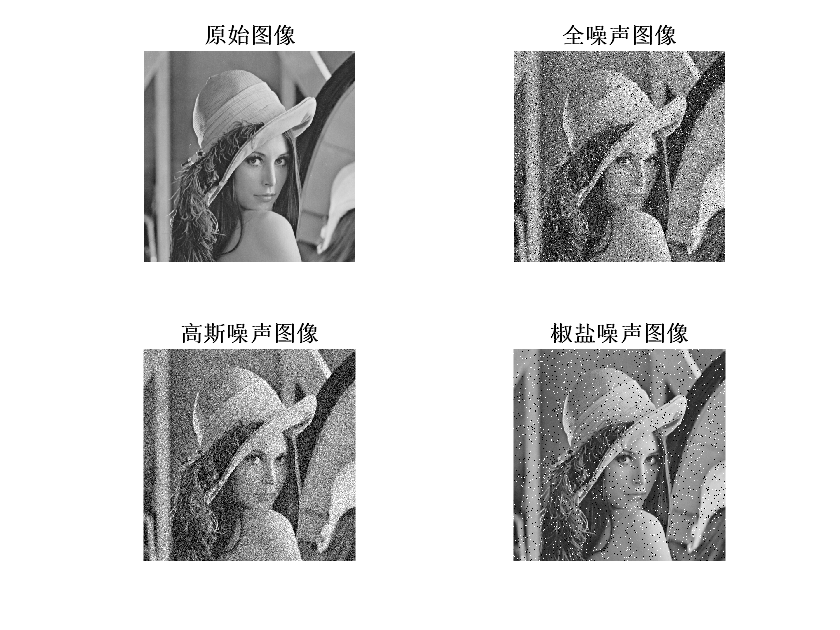
\includegraphics[width=0.9\textwidth]{image/result_subplot.png}
			\caption{四个子图}
			\label{subplot}
		\end{figure}
		\subsection{椒盐噪声的去噪}
		椒盐噪音中的噪声十分分散,并且噪声点的值都非常极端,要么全黑,
		要么全白,这时候用均值法就不能得到很好的效果,但是中值法却避开了这
		个问题,能对椒盐噪音进行很好的去噪。了解噪声的特点和成因,能让我们
		更好更快地选择去噪的方法,而不是盲目地尝试。于是
		我对椒盐噪声进行中值滤波处理,得到结果如下。
		\begin{figure}[H]
			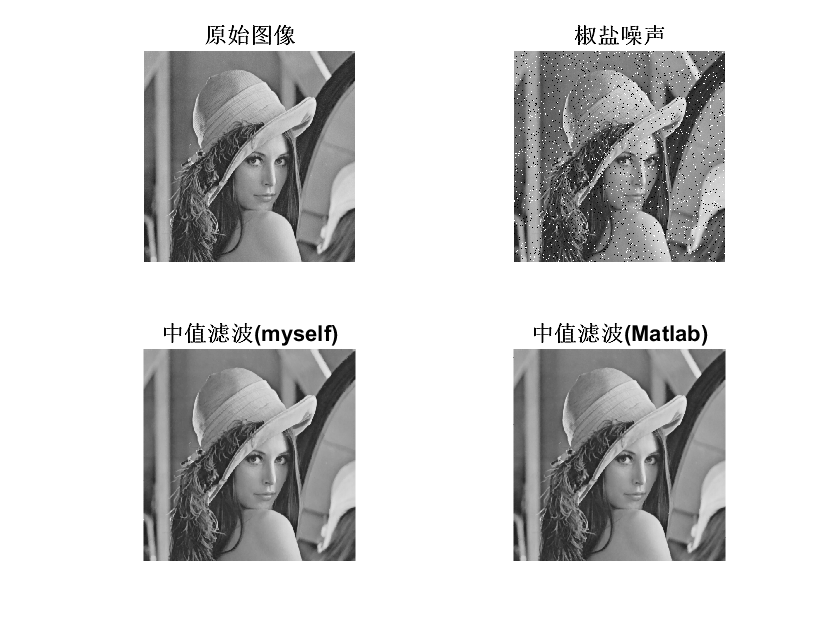
\includegraphics[width=\textwidth]{image/result_midfilter_salt.png}
			\caption{中值滤波处理椒盐噪声}
		\end{figure}
		
		同时返回误差
		\begin{figure}[H]
			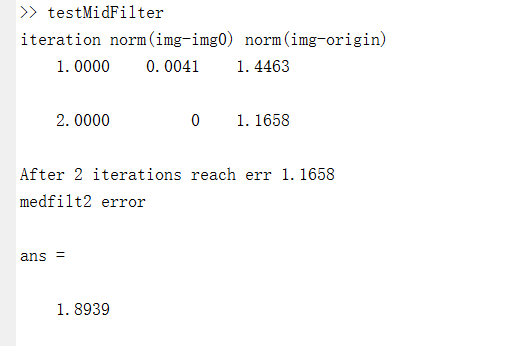
\includegraphics[width=\textwidth]{image/result_test_med1.png}
			\caption{中值滤波处理误差}
		\end{figure}
	
		可见对于椒盐噪声,我们使用中值滤波便可以很完美地进行除噪。无论是从视觉上,还是从运算结果上看,用中值处理椒盐噪声的效果效果相当好!
	
	\subsection{高斯噪声的去噪}
		对高斯噪声的去噪远没有椒盐噪声那么顺利得到比较好的结果,而且这方面比较棘手,于是试验了很多方法,试图得到更好的结果。结果发现采用AF滤波效果最好,但误差稍微还是有点大,AF算法的代码根据文献\cite{hal}中的源码改编而成。另外,根据实验结果,值得说明一点的是,在
		我使用的AF 算法是引用markus的成果.\cite{code},函数调用格式为
		$$sol = diffusionAnisotropic(img, varargin)$$
		
		主要有参数$sigma,sigmaGauss,maxIter,times$,于是在实际操作中我主要对$sigma$和$times$参数进行调整,并且发现$times$值不能太大,$sigma$应该取高斯噪声的方差,但在寻找AF算法最优参数时,发现如果$sigma = 0.0001$的效果还会略好于当$sigma$取该噪声的标准差,因为高斯噪声是均值为零方差为0.02(注意,matlab中的方差与一般文献中讨论的方差不一样),进行转换应该是$0.02\times 255 = 5.1$,具体原因还没弄清楚。
		
		
		\begin{longtable}{lll}
			方法&二范数&标准差\\
			\hline
			中值滤波&6.1975& 0.2307\\
			均值滤波&3.7342&0.1898\\
			维纳滤波&3.6922&0.1890\\
			AF滤波(sigma=5.1)&3.1787&0.1834\\
			AF滤波(sigma=0.0001)&3.0074& 0.1829\\
			\hline
			\caption{处理高斯噪声的几种方法}
		\end{longtable}
		\begin{figure}[H]
			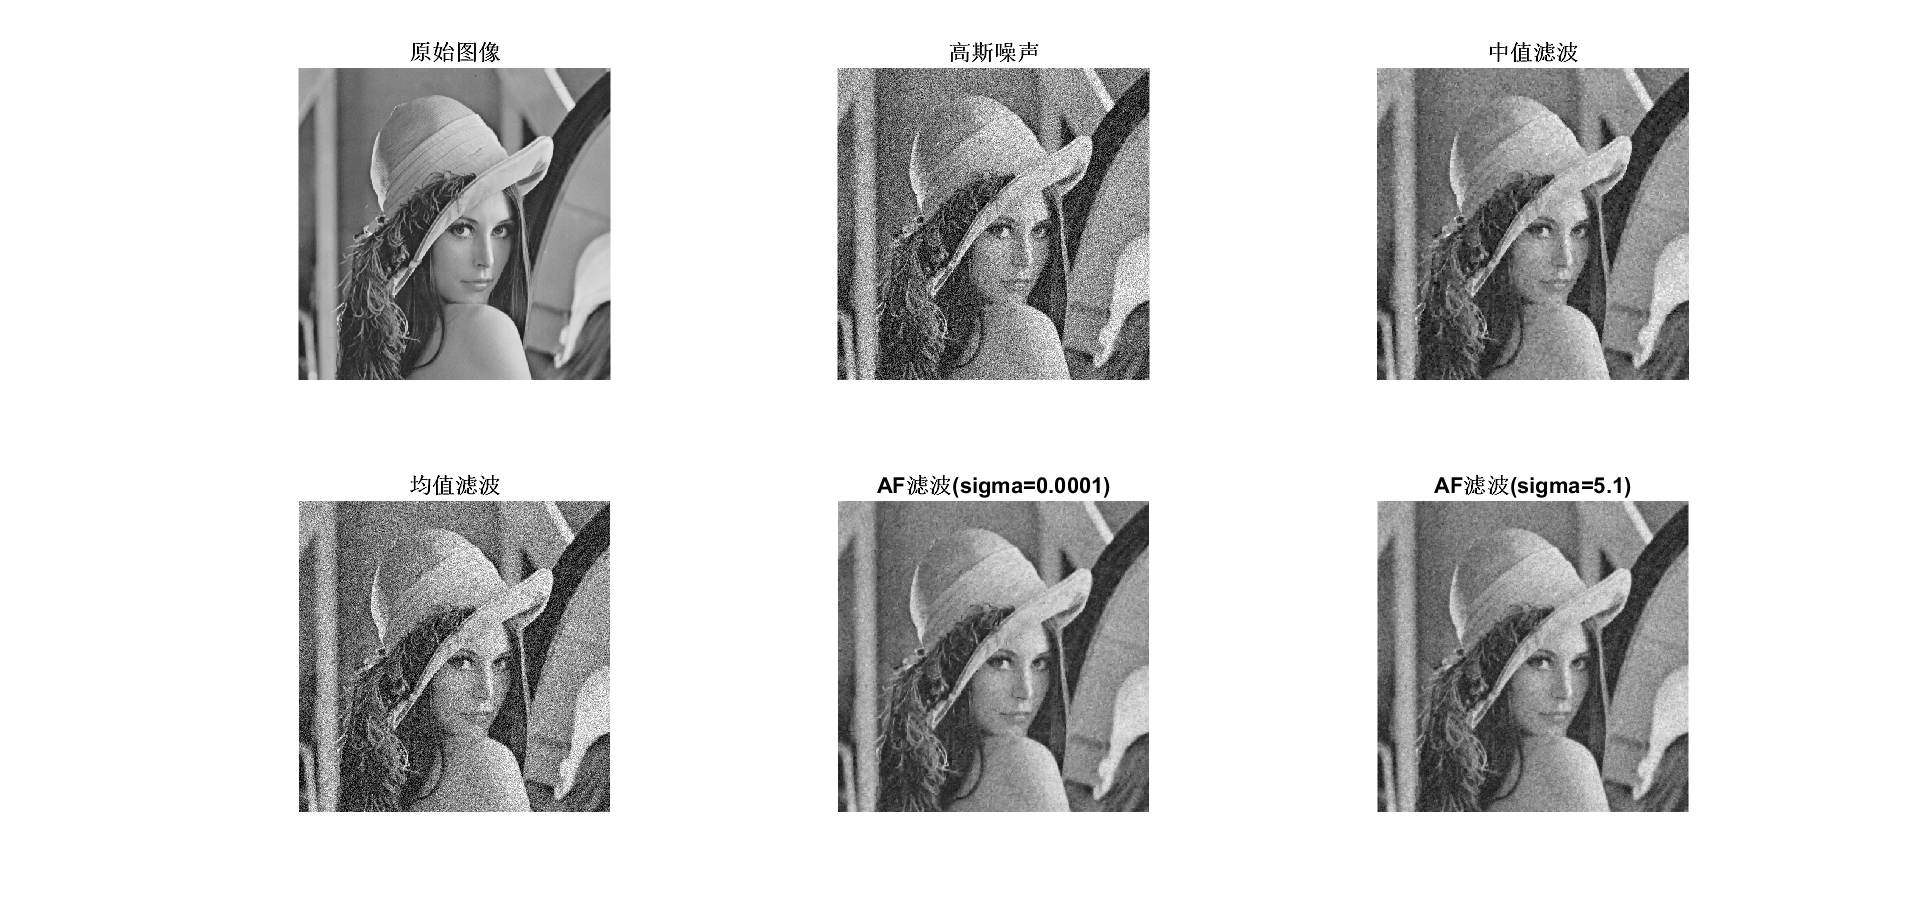
\includegraphics[width=\textwidth]{image/result_guass1.png}
			\caption{处理高斯噪声的几种方法}
		\end{figure}
		从上述运算结果即肉眼观察,可以判断采用AF滤波进行去噪的效果最好。
		\subsection{全噪声的去噪}
		在全噪声的去噪中,讨论了两种情况,分别是使用单一方法处理全噪声、以及使用混合方法处理全噪声
		
		\subsubsection{单一方法处理全噪声}
		\begin{longtable}{ll}
			\hline
			方法&二范数\\
			\hline
			中值滤波&6.5964\\
			均值滤波&9.6218\\
			维纳滤波&6.9799\\
			统计二维滤波&83.6541\\
			高斯滤波&9.6218\\
			AF滤波(sigma=5.1)&5.7530\\
			AF滤波(sigma=0.0001)&5.8173\\
			\hline
			\caption{单一方法处理全噪声}
		\end{longtable}
		\begin{figure}[H]
			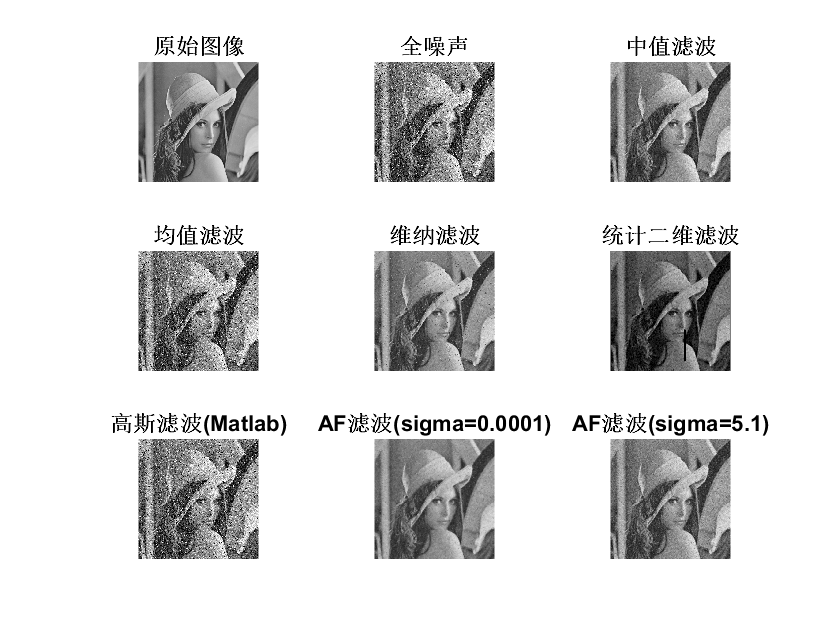
\includegraphics[width=\textwidth]{image/result_test_all2.png}
			\caption{单一方法处理全噪声}
		\end{figure}
		从上述运算结果以及肉眼观察可以判断用AF滤波进行去噪的效果最好。
		\subsubsection{混合方法处理全噪声}
		因为考虑到全噪声不是单一的高斯噪声,于是想组合几种方法来试试效果,但由于单一方法太多,组合多种多样,所以下面主要列出几种实验过程中效果比较好的几种组合
		\begin{longtable}{ll}
			\hline
			方法&二范数\\
			\hline
			中值滤波+均值滤波&6.2826\\
			中值滤波+AF滤波& 4.7857\\
			\hline
			\caption{混合方法处理全噪声}
		\end{longtable}
		\begin{figure}[H]
			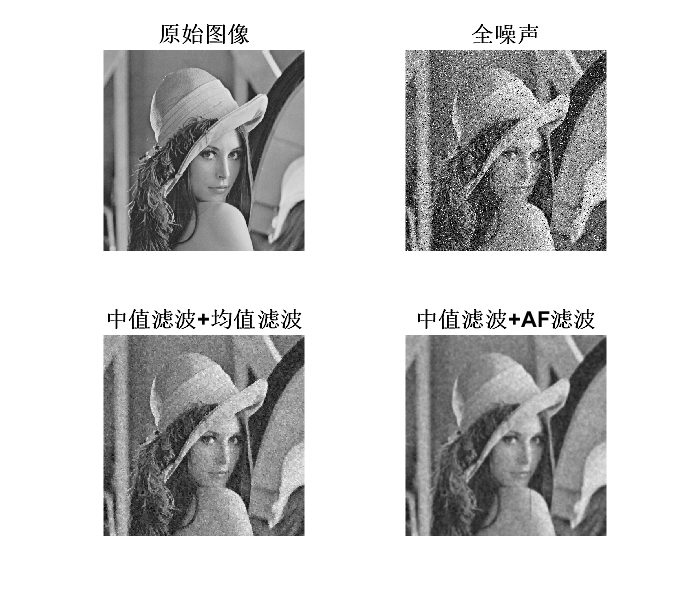
\includegraphics[width=\textwidth]{image/result_test_all3.png}
			\caption{混合方法处理全噪声}
		\end{figure}
		
		从上述运算结果和肉眼观察可以发现其实混合方法去噪效果也不是很好,或许也可能因为没有找到合适的组合,导致去噪效果没有单一方法去噪效果好。
		\section{结论}
		对于椒盐噪声,可以很有效地达到去噪效果,肉眼看跟原图毫无差别,此时跟原图差别二范数最低能够达到1.1658;对于高斯噪声,尝试的那些方法去噪效果不是很好,最好的是各向异性滤波方法,跟原图偏差的二范数最低能够达到3.0074;对于全噪声,因为有一部分是高斯噪声,所以对全噪声的去噪更加困难,尝试了一些方法,也尝试多种噪声相互结合使用,但最终效果都不是很好,跟原图差的二范数最低能达到4.7837.
	\begin{thebibliography}{99}
		\bibitem{hal}Antoni Buades, Bartomeu Coll, Jean-Michel Morel. A review of image denoising algorithms,
		with a new one. SIAM Journal on Multiscale Modeling and Simulation: A SIAM Interdisciplinary Journal, 2005, 4 (2), pp.490-530. <hal-00271141>
		\bibitem{wiki}https://en.wikipedia.org/wiki/Peak\_signal-to-noise\_ratio
		\bibitem{code}http://www5.informatik.uni-erlangen.de/en/our-team/mayer-markus
	\end{thebibliography}
\end{spacing}
	\section*{附录}
	\begin{appendices}
		%\section{Appendices}
		\textcolor[rgb]{0.98,0.00,0.00}{\textbf{subplot的代码:}}
		{\consolas\lstinputlisting{code/mysubplot.m}}
		\textcolor[rgb]{0.98,0.00,0.00}{\textbf{PSNR的计算代码:}}
		{\consolas\lstinputlisting{code/myPSNR.m}}
		\textcolor[rgb]{0.98,0.00,0.00}{\textbf{中值滤波的代码:}}
		{\consolas\lstinputlisting{code/myMidFilter.m}}
		\textcolor[rgb]{0.98,0.00,0.00}{\textbf{中值滤波的测试代码:}}
		{\consolas\lstinputlisting{code/testMidFilter(UTF8).m}}
		\textcolor[rgb]{0.98,0.00,0.00}{\textbf{均值滤波的代码:}}
		{\consolas\lstinputlisting{code/myAverageFilter.m}}
		\textcolor[rgb]{0.98,0.00,0.00}{\textbf{维纳滤波的代码:}}
		{\consolas\lstinputlisting{code/mywiener.m}}
		\textcolor[rgb]{0.98,0.00,0.00}{\textbf{AF滤波的代码:}}\cite{hal}
		{\consolas\lstinputlisting{code/diffusionAnisotropic.m}}
		%\textcolor[rgb]{0.98,0.00,0.00}{\textbf{PeronaMalik的代码:}}
		%{\consolas\lstinputlisting{code/diffusionPeronaMalik.m}}
		\par
		
	\end{appendices}
\end{document}

